\begin{frame}
  \frametitle{Probabilistic Property Evaluation (PPE)}
  \begin{block}{Property Violation Probability}
    \begin{figure}
      \centering
      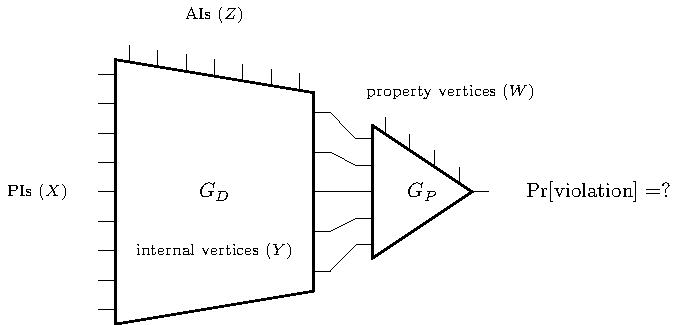
\includegraphics[scale=0.8]{fig/prob-design-eval/prob-spbn-miter.pdf}
    \end{figure}
    \pause
    \begin{itemize}
      \item PPE: the violation probability under $\pi:X\mapsto[0,1]$
            \pause
      \item MPPE: the maximum violation probability
    \end{itemize}
  \end{block}
\end{frame}

\begin{frame}
  \frametitle{Probabilistic Property Evaluation (PPE)}
  \begin{block}{Example: Probabilistic Equivalence Checking}
    \begin{figure}
      \centering
      \begin{circuitikz}[scale=0.4, transform shape]
    \tikzset{faulty/.style={muxdemux,muxdemux def={Lh=8,Rh=6,w=6,NL=7,NR=3,NB=0,NT=0},rotate=90}}
    \tikzset{golden/.style={muxdemux,muxdemux def={Lh=8,Rh=6,w=6,NL=4,NR=3,NB=0,NT=0},rotate=90}}
    \tikzset{black/.style={muxdemux,muxdemux def={Lh=1,Rh=0,w=1.5,NL=3,NR=1,NB=0,NT=0},rotate=90}}
    %\draw[step=1cm,gray,very thin] (-6,-6) grid (6,6); % For finding coordinates
    % Logic gates
    \node[faulty] (F) at (-2.5,-2) {};
    \node[golden] (G) at (2.5,-2) {};
    \node[xor port,rotate=90] (eq1) at (-2,1.7) {};
    \node[xor port,rotate=90] (eq2) at (0,1.7) {};
    \node[xor port,rotate=90] (eq3) at (2,1.7) {};
    \node[or port,rotate=90,number inputs=3] (and) at (0,3.5) {};
    \node[xor port,rotate=90,scale=0.5] (xor1) at (-3.5,-0.5) {};
    \node[black] (box1) at (-3.7,-2) {};
    \node[xor port,rotate=90,scale=0.5] (xor2) at (-1.5,-1) {};
    \node[black] (box2) at (-1.3,-2.5) {};
    % Wires
    \draw (F.rpin 1) -- (eq1.in 1);
    \draw (F.rpin 2) -- (eq2.in 1);
    \draw (F.rpin 3) -- (eq3.in 1);
    \draw (G.rpin 1) -- (eq1.in 2);
    \draw (G.rpin 2) -- (eq2.in 2);
    \draw (G.rpin 3) -- (eq3.in 2);
    \draw (eq1.out) -- (and.in 1);
    \draw (eq2.out) -- (and.in 2);
    \draw (eq3.out) -- (and.in 3);
    \draw (box1.rpin 1) -- ++(up:0.05cm) node{} -| (xor1.in 1);
    \draw (box2.rpin 1) -- ++(up:0.05cm) node{} -| (xor2.in 2);
    % Inputs
    \draw (F.lpin 1) -- ++(down:0.5cm) node{};
    \draw (F.lpin 2) -- ++(down:0.5cm) node{};
    \draw (F.lpin 3) -- ++(down:0.5cm) node{};
    \draw (G.lpin 1) -- ++(down:0.1cm) node[fill,circle,inner sep=1pt](c1){} -- ++(down:0.4cm){};
    \draw (c1) -| (F.lpin 4);
    \draw (G.lpin 2) -- ++(down:0.2cm) node[fill,circle,inner sep=1pt](c2){} -- ++(down:0.3cm){};
    \draw (c2) -| (F.lpin 5);
    \draw (G.lpin 3) -- ++(down:0.3cm) node[fill,circle,inner sep=1pt](c3){} -- ++(down:0.2cm){};
    \draw (c3) -| (F.lpin 6);
    \draw (G.lpin 4) -- ++(down:0.4cm) node[fill,circle,inner sep=1pt](c4){} -- ++(down:0.1cm){};
    \draw (c4) -| (F.lpin 7);
    % Labels
    \node at (-4,0) {$F$};
    \node at (4,0) {$G$};
    \node at (2.5,-5) {$X$};
    \node at (-3.75,-5) {$Z$};
    \node[font=\scriptsize] at (-3.25,-1.4) {$z_1$};
    \node[font=\scriptsize] at (-1.7,-1.9) {$z_2$};
\end{circuitikz}
    \end{figure}
    \pause
    \begin{itemize}
      \item PEC: the average difference probability under $\pi(x)=0.5$
            \pause
      \item MPEC: the maximum difference probability
    \end{itemize}
  \end{block}
\end{frame}

\begin{frame}
  \frametitle{Probabilistic Property Evaluation (PPE)}
  \begin{block}{Solving MPPE and PPE}
    \begin{itemize}
      \item MPPE
            \pause
            \begin{itemize}
              \item CNF-/BDD-based SSAT solving
                    \pause
            \end{itemize}
      \item PPE
            \pause
            \begin{itemize}
              \item Weighted model counting
                    \pause
              \item Unweighted model counting with formula rewriting
            \end{itemize}
    \end{itemize}
  \end{block}
\end{frame}

\begin{frame}
  \frametitle{Probabilistic Property Evaluation (PPE)}
  \begin{block}{Solving PPE and MPPE via SSAT}
    Given a miter SPBN $G_M$ and its CNF formula $\pf_M$:
    \pause
    \begin{itemize}
      \item PPE encoding
            \pause
            \belowdisplayskip=0pt
            \begin{align*}
              \alert<6>{\random{\pi(x_1)}x_1,\ldots,\random{\pi(x_n)}x_n},
              \random{p_{z_1}}z_1,\ldots,\random{p_{z_l}}z_l, \\
              \random{p_{w_1}}w_1,\ldots,\random{p_{w_q}}w_q,
              \exists y_1,\ldots,\exists y_m.
              \pf_M
            \end{align*}
            \pause
      \item MPPE encoding
            \pause
            \begin{align*}
              \alert<6>{\exists x_1,\ldots,\exists x_n},
              \random{p_{z_1}}z_1,\ldots,\random{p_{z_l}}z_l,
              \random{p_{w_1}}w_1,\ldots,\random{p_{w_q}}w_q,
              \exists y_1,\ldots,\exists y_m.
              \pf_M
            \end{align*}
    \end{itemize}
  \end{block}
\end{frame}

\begin{frame}
  \frametitle{BDD-Based SSAT Solving}
  {
    \small
    \begin{algorithmic}[1]
      \REQUIRE An ROBDD node $N$ and a prefix $Q$
      \ENSURE $\spb{N=\top}$ under $Q$
      \IF{($N$ is a terminal node)}\label{code:bddssat-recursive-constant-start}
      \RETURN $\nodesp{N}$\label{code:bddssat-recursive-constant-end}
      \ENDIF
      \IF{($\nodevisit{N}=\false$)}
      \IF{($Q(\nodevar{N})=\random{p}$)}
      \alert{\STATE $\nodesp{N}:=(1-p)\cdot\texttt{BddSsatRecur}(\nodeelse{N},Q)+p\cdot\texttt{BddSsatRecur}(\nodethen{N},Q)$}
      \label{code:bddssat-recursive-random}
      \ELSE
      \alert{\STATE $\nodesp{N}:=\max\{\texttt{BddSsatRecur}(\nodeelse{N},Q),\texttt{BddSsatRecur}(\nodethen{N},Q)\}$}
      \label{code:bddssat-recursive-exist}
      \ENDIF
      \STATE $\nodevisit{N} := \true$
      \ENDIF
      \RETURN $\nodesp{N}$
    \end{algorithmic}
  }
\end{frame}

\begin{frame}
  \frametitle{Probabilistic Property Evaluation (PPE)}
  \begin{block}{Connection between WMC and SSAT}
    $\random{p_{x_1}}x_1,\ldots,\random{p_{x_n}}x_n,\exists y_1,\ldots,\exists y_m.\pf$ is equivalent to a WMC instance of $\pf$ under $\wt(x_i)=p_{x_i}$ for every $x_i\in X$ if $X=\{x_1,\ldots,x_n\}$ is a \alert{base set} for $\pf$:
    \pause
    \begin{itemize}
      \item Base set: propagating values to variables outside the set
            \pause
            \begin{itemize}
              \item E.g., fresh variables for internal vertices during Tseitin transform
                    \pause
            \end{itemize}
      \item SSAT encoding of PPE can be solved by WMC
    \end{itemize}
  \end{block}
\end{frame}

\begin{frame}
  \frametitle{Probabilistic Property Evaluation (PPE)}
  \begin{block}{Rewriting WMC into Unweighted MC}
    \begin{itemize}
      \item Approximate model counting mostly focuses on unweighted instances
            \pause
      \item A rewriting technique to enjoy the advancements of approximate MC
            \pause
      \item Express a weight of the form $\frac{k}{2^n}$ with additional variables and clauses
    \end{itemize}
  \end{block}
  \pause
  \begin{block}{Example: WMC Rewriting}
    Express $p_{z_1}=0.25$ with $z_1\equiv z_2\land z_3$:
    \begin{figure}
      \centering
      \begin{circuitikz}[scale=0.7, transform shape]
    % Logic gates
    \node[and port] (y1) {$y_1'$};
    \node[xor port,right = of y1, anchor=in 1] (y3) {$y_3$};
    \node[or port,right = of y3, anchor=in 1] (y2) {$y_2$};
    \node[and port, below = of y1] (y4) {$y_4$};
    % Wires
    \draw (y1.out) -- (y3.in 1);
    \draw (y3.out) -- (y2.in 1);
    \draw (y4.out) -| (y3.in 2);
    % Labels
    \node[left = 0.1cm of y1.in 1] {$x_1$};
    \node[left = 0.1cm of y1.in 2] {$x_2$};
    \node[left = 0.1cm of y2.in 2] {$x_3$};
    \node[right = 0.1cm of y2.out] {$o$};
    \node[left = 0.1cm of y3.in 2] {$z_1$};
    \node[left = 0.1cm of y4.in 1] {$z_2$};
    \node[left = 0.1cm of y4.in 2] {$z_3$};
\end{circuitikz}
    \end{figure}
    \pause
    \begin{itemize}
      \item Unweighted: $p_{x_1}=p_{x_2}=p_{x_3}=p_{z_2}=p_{z_3}=0.5$
    \end{itemize}
  \end{block}
\end{frame}

\begin{frame}
  \frametitle{WMC Rewriting Procedure}
  {
    \scriptsize
    \begin{algorithmic}[1]
      \REQUIRE A formula $\pf$, a base set $\base$ for $\pf$,
      a wt. func. $\wt$ s.t. $\forall x\in\base.\wt(x)=\frac{k}{2^n}$
      \ENSURE A formula $\pf'$, a base set $\base'$ for $\pf'$,
      a wt. func. $\wt'$ s.t. $\forall x\in\base'.\wt'(x)=\frac{1}{2}$
      \STATE $\pf':=\pf,\base':=\base$
      \FORALL{($x\in\base$)}
      \STATE $var:=x,wt:=\wt(x)$
      \WHILE{($wt\neq\frac{1}{2}$)}
      \STATE $inv:=\bot$
      \IF{($wt>\frac{1}{2}$)}
      \STATE $wt:=1-wt,inv:=\top$
      \ENDIF
      \STATE $\pf':=\pf'\land((inv \oplus var) \equiv (y_{var} \land z_{var}))$
      \STATE $\base':=\base'\setminus\{var\}\cup\{y_{var}\}$
      \STATE $\wt'(y_{var})=\frac{1}{2}$
      \STATE $var=z_{var},wt=2 \cdot wt$
      \ENDWHILE
      \STATE $\base':=\base'\cup\{var\},\wt'(var)=\frac{1}{2}$
      \ENDFOR
      \RETURN $(\pf',\base',\wt')$
    \end{algorithmic}
  }
\end{frame}